The Square Kilometer Array (SKA) will be the largest radio-telescope of the 
world. Located in two different geographical areas (South-Africa and 
Australia/New Zealand) it will be one of the great physics machines of 21st 
Century and, when complete, one of the world’s engineering marvels. It will be 
constructed on different phases SKA1 (phase 1 2018-2023) and SKA2 (phase 2 
2023-2033). The development will be deployed using on two different pathfinders 
existing on each place (MeerKAT in South Africa and ASKAP in Australia). 
The SKA Telescope will be built on two different phases. The first one (SKA1)
starts at 2018 and is intended to provide the ~10\% of the total area at low and 
mid frequencies by 2023. The second phase (SKA2) has the goal to get the full
array working at low and mid frequencies by 2030. However, this timing schedule is
not the final decision and some changes could be applied for future versions.

The key science goals for this instrument are:

\begin{itemize}
	\item {Formation of the 1st galaxies in a dark Universe dominated by atomic gas.}
	\item {Evolution of the atomic gas till the current epoch.}
	\item {Strong Field Tests of Gravity Using Pulsars and Black Holes.}
	\item {Acceleration in the expansion of the Universe not understood yet.}
	\item {Habitable extra-solar planets (proto-planetary disks, biomarkers).}
\end{itemize}

It will be two different SKA facility locations depending on the frequency 
range for the sky observations. A common factor in both situations will be the 
huge number of antennas needed which require a high level accuracy 
synchronization. More information can be found in  
\cite{ska:baseline_description_v2}. 

%\begin{figure}[H]
%	\centering
%	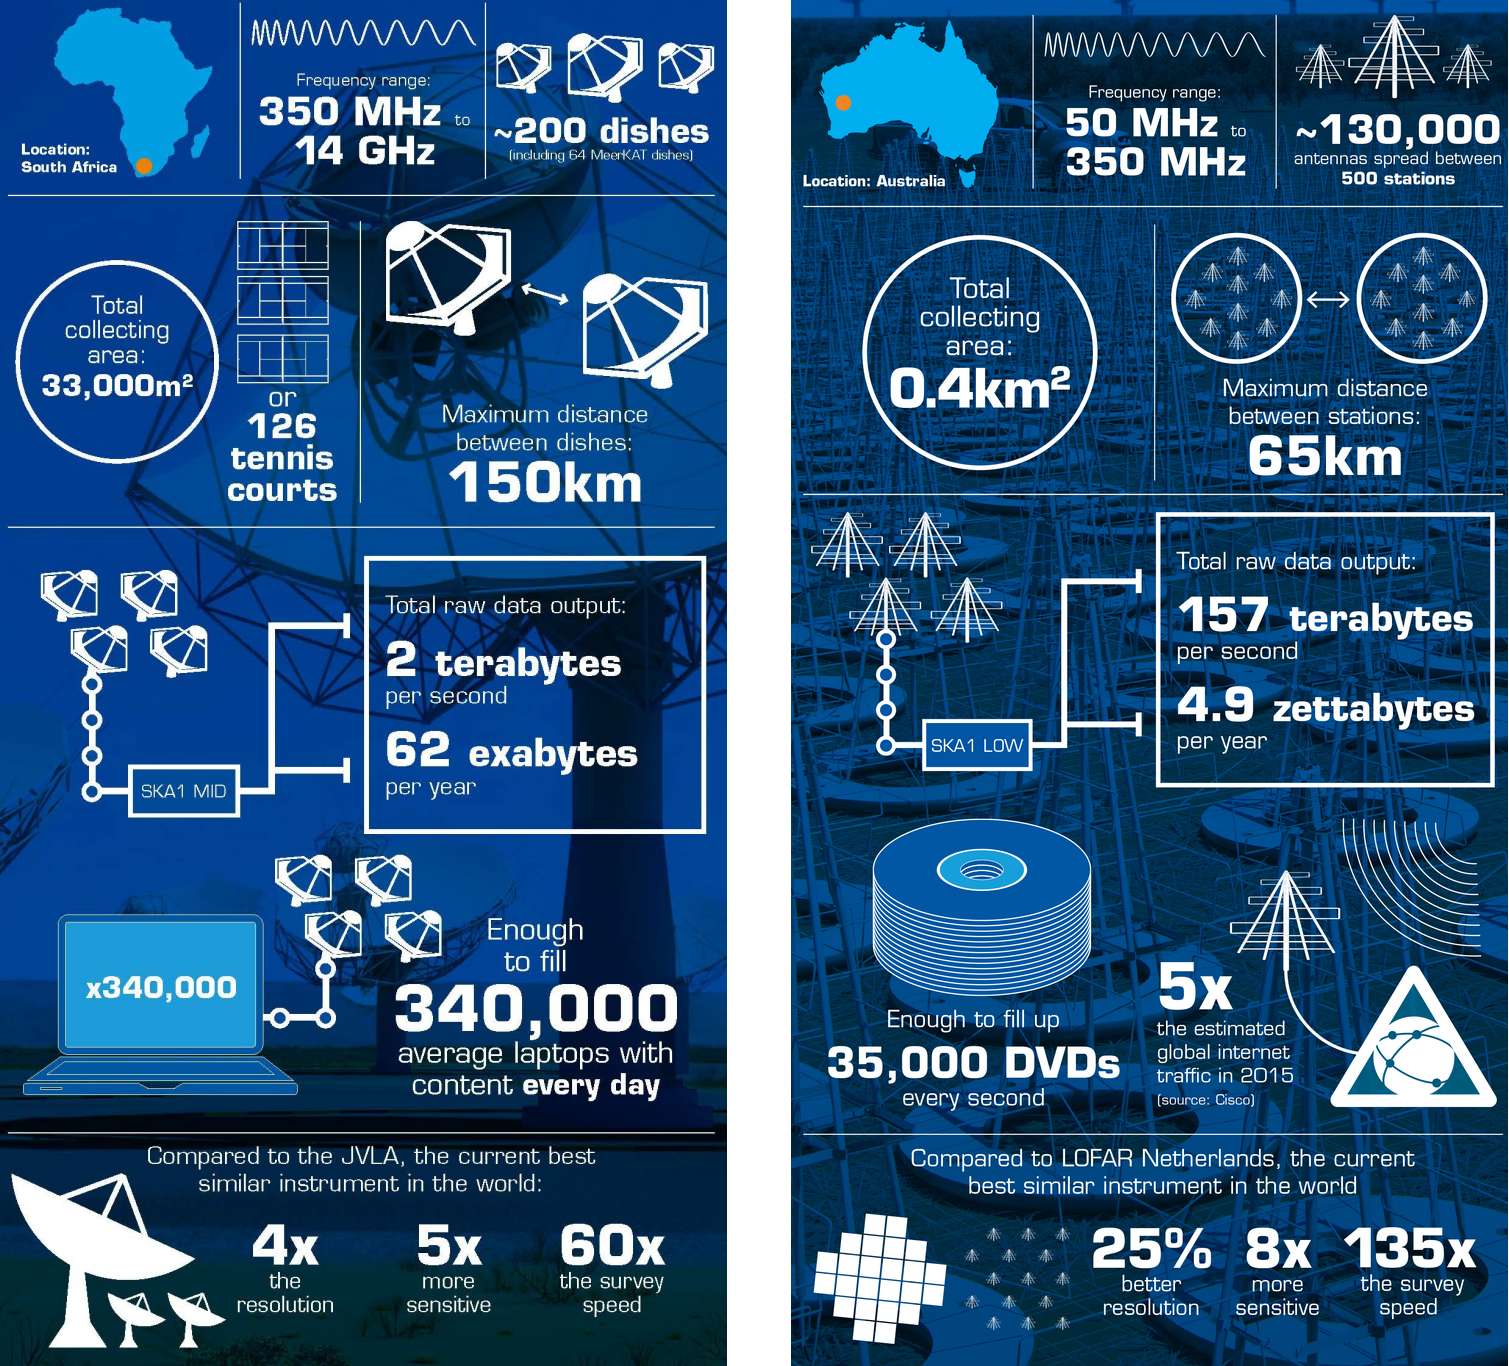
\includegraphics[scale=0.25]{img/ska_instruments}
%	\caption{The SKA's low frequency (right) and the mid-frequency (left) instruments.  SKA Telescope will be built on two different phases. These images (adapted from \cite{ska:multimedia_rsrcs}) illustrate key numbers corresponding to SKA1 phase (starting 2018). }
%	\label{fig:ska_instruments1}
%\end{figure}

%\missingfigure{The SKA Telescope instruments.}

%\klyonelnote{Al final, ¿Quitamos o dejamos esta figura?}

%The SKA1 telescope is being designed to optimize its performance and some key facts about both types of instruments are shown %on Fig. \ref{fig:ska_instruments1}. 

The scale of the SKA Telescope represents a huge leap forward in both 
engineering, research and development. The high performance specifications 
require the utilization of best technologies and design strategies possible and 
represent an unprecedented challenge for all the elements to be built. 

\subsection{SKA Telescope Network} \label{subsec:ska-telescope}

The SKA Telescope uses different types of networks to guarantee a proper operation of the infrastructure. The design of the network corresponds to the Signal and Data Transport (SaDT) element \cite{ska:sadt_website} and it includes all hardware and software necessary for the transmission of data and information between the Elements of the SKA. SADT also contains details about the provision of timing which is critical for interferometry.
The data network includes the Digital Data Backhaul (DDBH) that transports signals from the radio telescopes to the Central Signal Processor (CSP), and data products from the CSP to the Science Data Processor (SDP) and from the SDP to the regional SKA Data Centers. The total data rates are very high, approximately 80 Tb/s for the DDBH links and another 80Tb/s for the CSP links. 
Also covered by the SaDT is the Monitor and Control (M\&C) that transmits and receives monitoring and control information throughout the system and includes the Telescope Manager, itself comprised of three logical networks: Production Network, Engineering Network and Safety Network.

The final part of the SaDT is the Synchronization and Timing (SAT) that provides frequency and clock signals from a central clock ensemble to all elements of the system to maintain phase information to the required accuracy for all receptors, and timing signals for data identification and time critical activities at the receptors, and the CSP and SDP. To maintain phase coherence across the array requires short-term timing precision of around 1 ps, while for the requirements for the long-term timing for pulsar require 10 ns accuracies over 10 year periods. The timing is critical to the functionality of the SKA to work as a unified large telescope using a technique known as interferometry. This contribution will focus on the high accuracy synchronization method used for SKA responsible to provide a PPS (Pulse Per Second) signal to the critical elements. 

\begin{figure}[H]
	\centering
	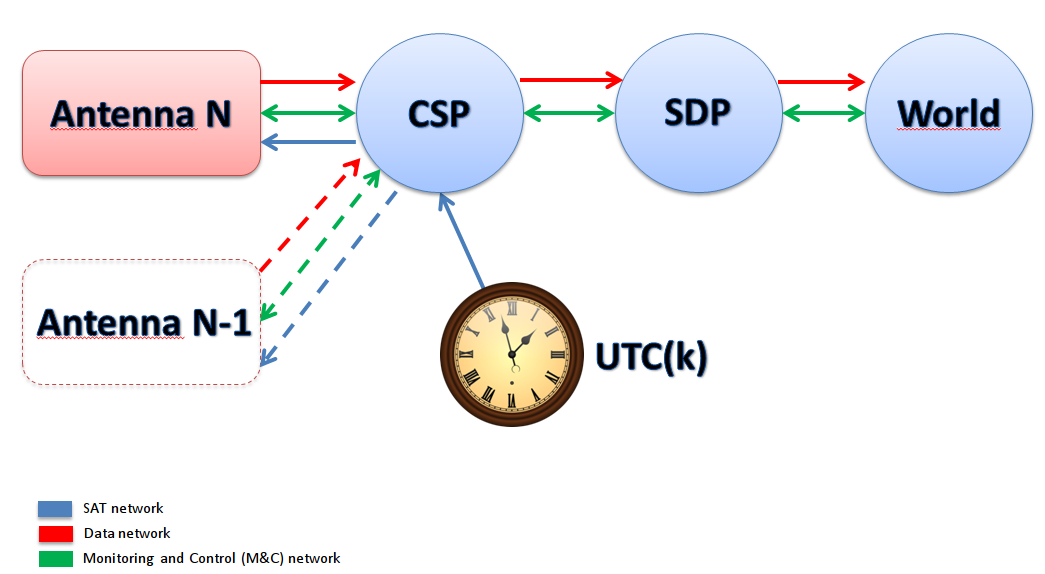
\includegraphics[scale=0.4]{img/ska_network_arch}
	\caption{The SKA Telescope network architecture is composed by three networks: the data network (red), the M\&C network (green) and the SAT network (blue). An external clock reference, UTC traceable, is provided to the whole Telescope elements in order of providing an unique time reference.}
	\label{fig:ska_net_arch1}
\end{figure}

%\missingfigure{The SKA Telescope network architecture figure.}

\subsection{Distribution of high accuracy timing signals for SKA1} \label{subsec:ska-distribution}

As determined by SaDT, SKA telescope should be able to distribute a common frequency reference to all the telescopes and, in addition, provides a uniform time reference to register all the events with ultra-high accuracy through time stamps. This task is done by the SAT (Synchronization and Timing) element that belongs to SaDT. The SKA timescale is maintained by the central clock ensemble for each telescope and will be steered to within designed limits of UTC (Coordinated Universal Time) and monitored with respect to UTC via GNSS time transfer techniques. These clock ensembles form the fundamental timescale for SKA and will be the basis for precision measurements of pulsars and other time-dependent phenomenas. As consequence, during this distribution, UTC refers to UTC (SKA), as realized by the central SKA clock ensemble.
This article will focus on the solutions to distribute the UTC time by means of PPS (Pulse-Per-Second signal). This PPS signal guarantees that all the scientific data are time-tag using a common reference. This time reference has high requirements coming from science that are not mandatory by other elements of the SKA systems as the monitor and control network. For these other elements, standard time transfer protocols as NTP or IEEE-1588 are a feasible solution. For the Telescope core, we illustrate that the high performance requirements imposed by the challenging scientific goals force to provide much more sophisticated approaches. 
The PPS distribution system will be in charge to deliver its output at the following locations:

\begin{itemize}
	\item {Each of the 133 dishes of SKA1-MID, and once to the Meerkat system. The maximum receptor baseline lengths are between 120-150 km.}
	\item {The core of SKA1-LOW, and the 45 stations in total along the 3 spiral arms. The maximum receptor baseline lengths are between 70-80 km. }
	\item {The encoded absolute time signal will be delivered to each of the three CSPs.}
\end{itemize}
 
Note that if the offset frequency scheme is to be applied to all SKA1-MID dishes, an additional 64 STFR endpoints will be needed in SKA1-MID. This provides between 182 and 246 endpoints to synchronize. 
The general array SAT requirements for the frequency distribution is 1 ps while the time synchronization and time-stamp requirement is 10ns. SaDT uses different mechanisms for achieving goals, frequency dissemination and PPS distribution. As consequence, because the goal in this contribution is just describing a solution for PPS distribution, the contribution work only considers the second requirement, the 10 ns synchronization as needed for example for the long-term timing Pulsar studies. Note that a complete description of the SKA network elements and topology is out of the scope of this contribution and only the requirements needed are presented to properly understand the need of the solution here developed. 
It is important to remark than the 10 ns requirement is allocated for the whole 
network. Because elements such as main clock also consume part of this, it 
translates into PPS-distribution time requirement of 5 ns. The error here 
includes PPS distribution, delay center precision, Dish timing transport and 
time-stamping errors and should be distributed on the different elements of the 
system that rely on the network topology that determine the number of hops. 
Based on current SAT network topology, the target specification for the 
elements of the PPS distribution system provides them an average time better 
than 2 ns. This is a quite challenging goal not only because impose a high 
accuracy synchronization goal but especially having into account the 
installation environmental conditions. The SKA1 use aerial optical fiber 
networks that are significantly affected by the large temperature excursion 
during operation, more than 20º due to the installation on desert locations of 
Sud-Africa and Australia. Furthermore the outdoor wind velocities during normal 
operation could achieve up to 40 km/h. it makes the fibers oscillate, changing 
their length, which must be compensated on real-time during execution or 
averaged them out. 

Next section will provide the description of the solution proposed to be use on SKA telescope as mechanism for PPS distribution. 
